% generated by Docutils <http://docutils.sourceforge.net/>
\documentclass[a4paper,english]{article}
\usepackage{fixltx2e} % LaTeX patches, \textsubscript
\usepackage{cmap} % fix search and cut-and-paste in PDF
\usepackage{babel}
\usepackage[T1]{fontenc}
\usepackage[latin1]{inputenc}
\usepackage{ifthen}
\usepackage{graphicx}





% Added by Mike

\usepackage[margin=1in]{geometry}
\usepackage{listings}
\lstset{language=XML}
\lstset{% general command to set parameter(s)
basicstyle=\footnotesize, % print whole listing small
%basicstyle=\footnotesize, % print whole listing small
keywordstyle=\color{blue}, %\bfseries\underbar,
% underlined bold black keywords
identifierstyle=, % nothing happens
commentstyle=\color{OliveGreen}, % white comments
stringstyle=\ttfamily, % typewriter type for strings
showstringspaces=false, % no special string spaces
language=matlab,
frame=lines,
float=tbfh}





%%% User specified packages and stylesheets

%%% Fallback definitions for Docutils-specific commands

% admonition (specially marked topic)
\providecommand{\DUadmonition}[2][class-arg]{%
  % try \DUadmonition#1{#2}:
  \ifcsname DUadmonition#1\endcsname%
    \csname DUadmonition#1\endcsname{#2}%
  \else
    \begin{center}
      \fbox{\parbox{0.9\textwidth}{#2}}
    \end{center}
  \fi
}

% title for topics, admonitions and sidebar
\providecommand*{\DUtitle}[2][class-arg]{%
  % call \DUtitle#1{#2} if it exists:
  \ifcsname DUtitle#1\endcsname%
    \csname DUtitle#1\endcsname{#2}%
  \else
    \smallskip\noindent\textbf{#2}\smallskip%
  \fi
}

% titlereference role
\providecommand*{\DUroletitlereference}[1]{\textsl{#1}}

% hyperlinks:
\ifthenelse{\isundefined{\hypersetup}}{
  \usepackage[colorlinks=true,linkcolor=blue,urlcolor=blue]{hyperref}
}{}
\hypersetup{
  pdftitle={The NineML Abstraction Layer \& Object Model},
}

%%% Body
\begin{document}

% Document title
\title{The NineML Abstraction Layer \& Object Model%
  \phantomsection%
  \label{the-nineml-abstraction-layer-object-model}}
\author{}
\date{}
\maketitle


%___________________________________________________________________________

\section*{Introduction%
  \phantomsection%
  \addcontentsline{toc}{section}{Introduction}%
  \label{introduction}%
}

NineML is an API designed for specifying the dynamics and connectivity of neural
simulations; in particular for large-scale simulations of many point neurons.
NineML is split into two levels; User Layer and Abstraction Layer.
Simplistically, the abstraction layer allows us to define the behaviour of
\emph{parameterised} components, while the user layer defines the instantiation of
these components in terms of parameters and interconnectivity.

The NineML abstraction is an evolving standard. There are currently three
implementations; in Python, Java (via LEMS/NEUROML??) and Chicken.

In this document we define the concepts common to the object models supported by
these three implementations.


%___________________________________________________________________________

\section*{The Object Model%
  \phantomsection%
  \addcontentsline{toc}{section}{The Object Model}%
  \label{the-object-model}%
}

In the NineML Abstraction Layer; we define our model in terms of \textbf{ComponentClasses}. A \textbf{ComponentClass} could typically represent a point-neuron model or a synapse model for example.

A \textbf{ComponentClass} is composed of its \textbf{Interface} and its \textbf{Dynamics}.


%___________________________________________________________________________

\subsection*{Dynamics%
  \phantomsection%
  \addcontentsline{toc}{subsection}{Dynamics}%
  \label{dynamics}%
}

The Dynamics are the \emph{internal} mechanisms governing the behaviour of the component.
The dynamics of a component are specified in terms of the following:
%
\begin{itemize}

\item \textbf{StateVariables}

\item A \emph{RegimeGraph} composed of \textbf{Regimes} \& \textbf{Transitions}

\item \textbf{Aliases}

\end{itemize}


%___________________________________________________________________________

\subsubsection*{The \emph{RegimeGraph} and StateVariables%
  \phantomsection%
  \addcontentsline{toc}{subsubsection}{The RegimeGraph and StateVariables}%
  \label{the-regimegraph-and-statevariables}%
}

The internal state of a component is defined by a set of \textbf{StateVariables}; variables that can
change either continuously or discontinuously as a function of time.

The \textbf{Regimes} form the vertices and the \textbf{Transitions} form the directional edges of the \emph{RegimeGraph}, which must have at least one \textbf{Regime}, and contain no regime-islands.  At any given time, a component will be in a single \textbf{Regime}, and can change which \textbf{Regime} it is in through \textbf{Transitions}.

A \textbf{Regime} contains a set of \textbf{TimeDerivatives}, one for each \textbf{StateVariable} of the \textbf{ComponentClass}, which define how the \textbf{StateVariables} evolve over time.

The \textbf{StateVariable} changes happen in two ways:
%
\begin{quote}
%
\begin{itemize}

\item continuously through \textbf{TimeDerivatives} (in \textbf{Regimes}), which define the \textbf{StateVariables}
evolution over time, for example \DUroletitlereference{dX/dt=1-X}

\item discretely through \textbf{StateAssignments} (in \textbf{Transitions}), which make discrete changes to a
\textbf{StateVariable}'s value, for example \DUroletitlereference{X = X + 1}

\end{itemize}

\end{quote}

This diagram shows the dynamics block for an example component.

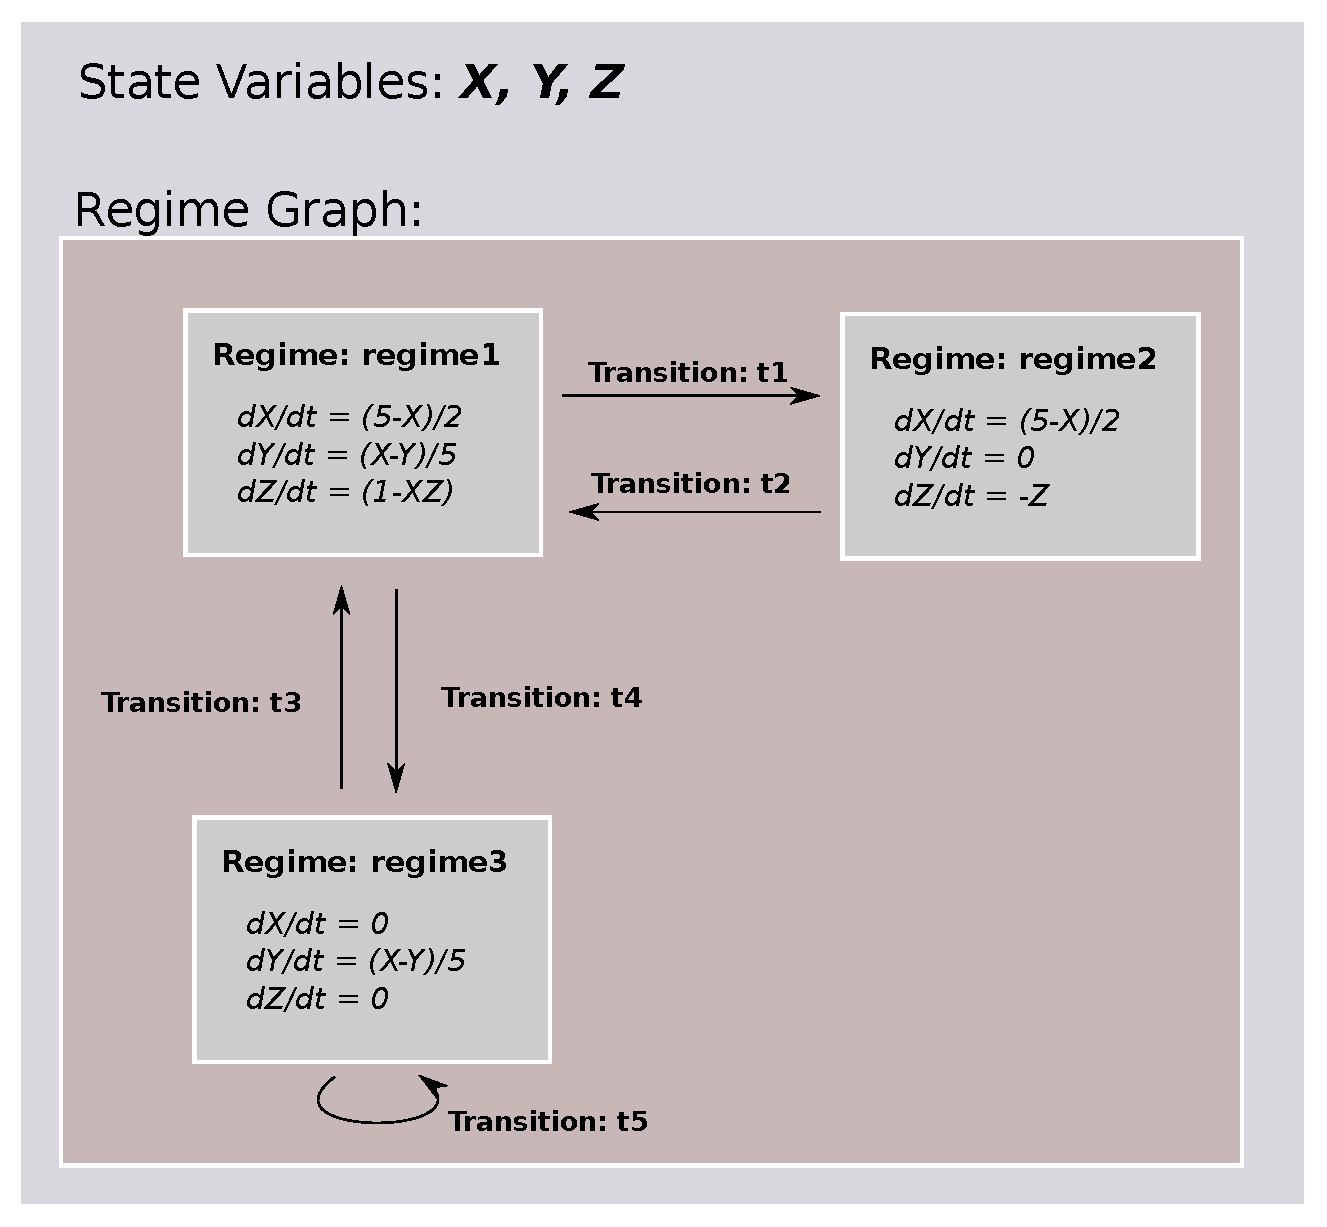
\includegraphics{al_figs/SimpleRegimeGraph.eps}

This dynamics has 3 state variables, \emph{X,Y \& Z}, and a state graph with 3
regimes, \emph{regime1}, \emph{regime2} \& \emph{regime3}. At any time, a component will be in one of these regimes, and the state variables will evolve accordingly.

Movement between \textbf{Regimes} happens via \textbf{Transitions}. There are 2 types of
Transitions:
%
\begin{itemize}

\item An \textbf{OnCondition} function of the \textbf{StateVariables}, for example \DUroletitlereference{X>Y}.

\item An \textbf{OnEvent} on an input \textbf{EventPort}. (Discussed further in XX).

\end{itemize}

During either type of transition; three things can happen:
%
\begin{itemize}

\item The component can change regime. For example, in the example above, if the
component is in \emph{regime3}, and the trigger for \emph{t3} is satisfied, then the
component will move into \emph{regime1}.

\item \textbf{StateAssignments} can take place, for example, \DUroletitlereference{X=0}

\item The component can send \textbf{OutputEvents}

\end{itemize}

During a transition, multiple \textbf{StateAssignments} and \textbf{OutputEvents} can occur.
(For more on the resolution of \textbf{Transitions}, see XX)

\DUadmonition[note]{
\DUtitle[note]{Note}
%
\begin{itemize}

\item If a \textbf{TimeDerivative} for a \textbf{StateVariable} is not defined in a \textbf{Regime}, it is
assumed to be zero.

\item A \textbf{Transition} does not need to lead to a change of \textbf{Regime}. It can cause
\textbf{StateAssignments} and/or \textbf{OutputEvents}, and return to the original
regime. (For example \emph{t5} in the diagram)

\end{itemize}
}


%___________________________________________________________________________

\subsubsection*{Aliases%
  \phantomsection%
  \addcontentsline{toc}{subsubsection}{Aliases}%
  \label{aliases}%
}

\textbf{Aliases} are motivated from two problems;
%
\begin{itemize}

\item Rather than writing long expressions for functions of \textbf{StateVariables}, we can
define an \textbf{Alias} once.
For example, we can define chains of \textbf{Aliases}:
%
\begin{quote}{\ttfamily \raggedright \noindent
m\_alpha~=~(alphaA~+~alphaB*V)~/~(~alphaC~+~exp((alphaD+V/alphaE))~)\\
m\_beta~=~~(betaA~+~betaB*V)~/~(~betaC~+~exp((betaD+V/betaE))~)\\
minf~=~m\_alpha~/~(m\_alpha~+~m\_beta)\\
mtau~=~1./(m\_alpha+m\_beta)\\
dm/dt~=~(1/C)~*~(minf-m)/mtau
}
\end{quote}

In this case, \emph{m\_alpha}, \emph{m\_beta}, \emph{minf} and \emph{mtau} are all alias
definitions. There is no reason we couldn't expand our \DUroletitlereference{dm/dt}
description out to eliminate these intermediate \textbf{Aliases}, but the expression
would be very long and difficult to read.

\item If we would like to communicate a value other than a simple \textbf{StateVariable} to
to another \textbf{ComponentClass}. For example, if we have a component representing a
neuron, which has an internal \textbf{StateVariable}, 'V', we may be interested in
transmitting a current, for example \DUroletitlereference{i=g*(E-V)}.

\end{itemize}

\DUadmonition[note]{
\DUtitle[note]{Note}

Aliases are defined in the Dynamics, \emph{not} in the Regime. This means that
aliases are the same across all regimes.
}


%___________________________________________________________________________

\subsubsection*{Events%
  \phantomsection%
  \addcontentsline{toc}{subsubsection}{Events}%
  \label{events}%
}

As well as being able to communicate continuous values, components are also able
to emit and receive \textbf{Events}. Events are discrete notifications that are transmitted
over EventPorts. Since EventPorts have names, saying
that we transmit  'event1' for example would mean transmitting an event on
the EventPort called 'event1'. Events can be used to signal action
potentials firing for example.


%___________________________________________________________________________

\subsection*{Interface%
  \phantomsection%
  \addcontentsline{toc}{subsection}{Interface}%
  \label{interface}%
}

The interface is the \emph{external} view of the component; what inputs and outputs the component exposes
to other components and the parameters that can be set for the component.

The interface consists of \emph{Ports} and \emph{Parameters}.


%___________________________________________________________________________

\subsubsection*{Parameters%
  \phantomsection%
  \addcontentsline{toc}{subsubsection}{Parameters}%
  \label{parameters}%
}

Parameters allow us to define the dynamics of a component once, then adjust the
behaviours by using different parameters. For example, if we are building an
integrate-and-fire neuron, we can specify that the Reset-Voltage and the
Firing-Threshold are parameters, write our dynamics in terms of these
parameters, then use the \emph{User Layer} to provide parameters to create different
neurons. Parameters are set at the start of the simulation, and remain constant
throughout.


%___________________________________________________________________________

\subsubsection*{Ports%
  \phantomsection%
  \addcontentsline{toc}{subsubsection}{Ports}%
  \label{ports}%
}

Ports allow components to communicate between each other during a simulation.
There are 2 types, \emph{AnalogPorts} and \emph{EventPorts}, and each can have
different modes.


%___________________________________________________________________________

\paragraph*{AnalogPorts%
  \phantomsection%
  \addcontentsline{toc}{paragraph}{AnalogPorts}%
  \label{analogports}%
}

AnalogPorts transmit and receive continuous values, either  \textbf{Aliases} and
\textbf{StateVariables}. AnalogPorts can have 3 modes:
%
\begin{quote}
%
\begin{itemize}

\item \texttt{SendPort} - transmit data originating in this component which can be read by
other components.

\item \texttt{RecvPort} - receive data from another components \texttt{SendPort} port.
Each \texttt{RecvPort} can be connected to \emph{one} \texttt{SendPort}.

\item \texttt{ReducePort} - receive data from multiple \texttt{SendPort} . These
differ from \texttt{RecvPorts} in that they can be connected to multiple
\texttt{SendPort} . \texttt{ReducePorts} take an additional operator,
\texttt{reduce\_op}, which specifies how the data from multiple \texttt{Send}
ports should be combined to produce a single value. Currently, the
only supported operations is \DUroletitlereference{+}, which sums the inputs. The
motivation for \texttt{ReducePorts} is that it allows us to make our
component definitions more general. For example, if we are defining a
neuron, would define a \texttt{ReducePort} called, \texttt{InjectedCurrents}.
This allows us to write the membrane equation for that neuron as
\DUroletitlereference{dV/dt = (1/C) * InjectedCurrents}

Then, when we connect this neuron to synapses, current-clamps, etc, we
simply need to connect the SendPorts containing the currents of these components onto
the \texttt{InjectedCurrents} reduce-port, within having to change our
original component definitions.

\end{itemize}

\end{quote}


%___________________________________________________________________________

\paragraph*{EventPorts%
  \phantomsection%
  \addcontentsline{toc}{paragraph}{EventPorts}%
  \label{eventports}%
}

Event ports transmit discrete events. They are useful for example in
simulation of integrate-and-fire neurons to notify components about neuron's
spiking. Event ports only have 2 modes:
%
\begin{quote}
%
\begin{itemize}

\item \texttt{SendPort} - transmit events originating in this component which can be read by
other components

\item \texttt{RecvPort} - receive events from another components \texttt{SendPort} port.
Each recv port can be connected to \emph{multiple} \texttt{SendPort}.

\end{itemize}

\end{quote}

For example, a synapse component may have a \texttt{RecvPort} connected to the
presynaptic neurons \texttt{SendPort} port. When the presynaptic neuron fires;
it delivers an event to the synapse, which could cause it to produce current
flow in a post-synaptic neuron.


\pagebreak


%___________________________________________________________________________

\section*{NineML Abstraction Layer as XML%
  \phantomsection%
  \addcontentsline{toc}{section}{NineML Abstraction Layer as XML}%
  \label{nineml-abstraction-layer-as-xml}%
}


%___________________________________________________________________________

\subsection*{Tag Descriptions%
  \phantomsection%
  \addcontentsline{toc}{subsection}{Tag Descriptions}%
  \label{tag-descriptions}%
}


%___________________________________________________________________________

\subsubsection*{<NineML>%
  \phantomsection%
  \addcontentsline{toc}{subsubsection}{<NineML>}%
  \label{nineml}%
}
%
\begin{lstlisting}
<NineML>
\end{lstlisting}

This is the root namespace tag for a NineML file. It can contain
\DUroletitlereference{<ComponentClass>} elements.


%___________________________________________________________________________

\subsubsection*{<ComponentClass>%
  \phantomsection%
  \addcontentsline{toc}{subsubsection}{<ComponentClass>}%
  \label{componentclass}%
}
%
\begin{lstlisting}
<ComponentClass name="">
\end{lstlisting}


This tag starts an abstraction layer component definition.

Attributes:
%
\begin{itemize}

\item name {[}Required{]}

\end{itemize}

Child Elements:
%
\begin{itemize}

\item <Parameter> {[}0+{]}

\item <AnalogPort>{[}0+{]}

\item <EventPort> {[}0+{]}

\item <Dynamics>  {[}1{]}

\end{itemize}


%___________________________________________________________________________

\subsubsection*{<Parameter>%
  \phantomsection%
  \addcontentsline{toc}{subsubsection}{<Parameter>}%
  \label{parameter}%
}
%
\begin{lstlisting}
<Parameter name="" dimension="">
\end{lstlisting}

This tag specifies a parameter in the interface of the component

Attributes:
%
\begin{itemize}

\item name {[}Required{]}

\item dimension {[}Required{]}

\end{itemize}

Child Elements: \texttt{None}


%___________________________________________________________________________

\subsubsection*{<AnalogPort>%
  \phantomsection%
  \addcontentsline{toc}{subsubsection}{<AnalogPort>}%
  \label{analogport}%
}
%
\begin{lstlisting}
<AnalogPort name="" mode="" reduce_op="" dimension=" >
\end{lstlisting}

This tag specifies an AnalogPort in the interface of the component

Attributes:
%
\begin{itemize}

\item name {[}Required{]}

\item mode {[}Required: 'send','recv' or 'reduce'{]}

\item reduce\_op {[}Required if mode=='reduce'{]}

\item dimension {[}Required{]}

\end{itemize}

Child Elements: \texttt{None}


%___________________________________________________________________________

\subsubsection*{<EventPort>%
  \phantomsection%
  \addcontentsline{toc}{subsubsection}{<EventPort>}%
  \label{eventport}%
}
%
\begin{lstlisting}
<EventPort name="" mode="">
\end{lstlisting}

This tag specifies an EventPort in the interface of the component

Attributes:
%
\begin{itemize}

\item name {[}Required{]}

\item mode {[}Required: 'send','recv'{]}

\item dimension {[}Required{]}

\end{itemize}

Child Elements: \texttt{None}


%___________________________________________________________________________

\subsubsection*{<Dynamics>%
  \phantomsection%
  \addcontentsline{toc}{subsubsection}{<Dynamics>}%
  \label{id1}%
}
%
\begin{lstlisting}
<Dynamics>
\end{lstlisting}

This tag specifies the dynamics of the component

Attributes: \texttt{None}

Child Elements:
%
\begin{itemize}

\item <StateVariable> {[}0+{]}

\item <Alias> {[}0+{]}

\item <Regime> {[}1+{]}

\end{itemize}


%___________________________________________________________________________

\subsubsection*{<StateVariable>%
  \phantomsection%
  \addcontentsline{toc}{subsubsection}{<StateVariable>}%
  \label{statevariable}%
}
%
\begin{lstlisting}
<StateVariable name="" dimension="">
\end{lstlisting}

This tag declares a state-variable in the component

Attributes:
%
\begin{itemize}

\item name {[}Required{]} (The variable name)

\item dimension {[}Required{]}

\end{itemize}

Child Elements: \texttt{None}


%___________________________________________________________________________

\subsubsection*{<Alias>%
  \phantomsection%
  \addcontentsline{toc}{subsubsection}{<Alias>}%
  \label{alias}%
}
%
\begin{lstlisting}
<Alias name="">
\end{lstlisting}

This tag declares an alias in the component

Attributes:
%
\begin{itemize}

\item name {[}Required{]} (The alias name)

\item dimension {[}Required{]}

\end{itemize}

Child Elements:
%
\begin{itemize}

\item <MathInline> {[}Required{]} (The equation on the right-hand-side of the alias)

\end{itemize}


%___________________________________________________________________________

\subsubsection*{<Regime>%
  \phantomsection%
  \addcontentsline{toc}{subsubsection}{<Regime>}%
  \label{regime}%
}
%
\begin{lstlisting}
<Regime name="">
\end{lstlisting}

This tag declares an regime in the component. There must be exactly on
TimeDerivative block for each StateVariable block declared in the enclosing
<Dynamics> block, even if it has a RHS of zero.

Attributes:
%
\begin{itemize}

\item name {[}Required{]} (The regime name)

\end{itemize}

Child Elements:
%
\begin{itemize}

\item <TimeDerivative> {[}0+{]}

\item <OnCondition> {[}0+{]} (The transitions from this regime, triggered by conditions)

\item <OnEvent> {[}0+{]} (The transitions from this regime, triggered by events)

\end{itemize}


%___________________________________________________________________________

\subsubsection*{<TimeDerivative>%
  \phantomsection%
  \addcontentsline{toc}{subsubsection}{<TimeDerivative>}%
  \label{timederivative}%
}
%
\begin{lstlisting}
<TimeDerivative variable="">
\end{lstlisting}

This tag defines the differential equation controlling the evolution of a StateVariable while
in this regime.

Attributes:
%
\begin{itemize}

\item variable {[}Required{]} (The name of the state variable)

\end{itemize}

Child Elements:
%
\begin{itemize}

\item <MathInline> {[}1{]} (The right-hand-side of the differential equation)

\end{itemize}


%___________________________________________________________________________

\subsubsection*{<OnCondition>%
  \phantomsection%
  \addcontentsline{toc}{subsubsection}{<OnCondition>}%
  \label{oncondition}%
}
%
\begin{lstlisting}
<OnCondition>
\end{lstlisting}

This block specifies a transition from the enclosing Regime, which is triggered
by a mathematical function of the Component's Aliases, StateVariables, Ports and
Parameters.

Attributes: \texttt{None}

Child Elements:
%
\begin{itemize}

\item %
\begin{description}
\item <Trigger> {[}1{]} (A <Trigger> block defining the condition that causes this transition to occur)

\end{description}

\item <StateAssignment> {[}0+{]} (The state assignments that should occur when this
transition is triggered)

\item <EventOut> {[}0+{]} (The events that should be sent when this transition is triggered)

\end{itemize}


%___________________________________________________________________________

\subsubsection*{<OnEvent>%
  \phantomsection%
  \addcontentsline{toc}{subsubsection}{<OnEvent>}%
  \label{onevent}%
}
%
\begin{lstlisting}
<OnEvent port="">
\end{lstlisting}

This block specifies a transition from the enclosing Regime, which is triggered
by an input event.

Attributes:
%
\begin{itemize}

\item port {[}Required{]} The name of the input event port which triggers this
transition

\end{itemize}

Child Elements:
%
\begin{itemize}

\item <StateAssignment> {[}0+{]} (The state assignments that should occur when this
transition is triggered)

\item <EventOut> {[}0+{]} (The events that should be sent when this transition is triggered)

\end{itemize}


%___________________________________________________________________________

\subsubsection*{<Trigger>%
  \phantomsection%
  \addcontentsline{toc}{subsubsection}{<Trigger>}%
  \label{trigger}%
}
%
\begin{lstlisting}
<Trigger>
\end{lstlisting}

This block is used by <OnCondition> blocks to define the condition needed for
them to be triggered.

Attributes: \texttt{None}

Child Elements:
%
\begin{itemize}

\item <MathInline> {[}1{]} (A mathematical expression. This should evaluate to a
boolean, for example by invoking a comparison operator  \DUroletitlereference{('>', '<')} )

\end{itemize}


%___________________________________________________________________________

\subsubsection*{<StateAssignment>%
  \phantomsection%
  \addcontentsline{toc}{subsubsection}{<StateAssignment>}%
  \label{stateassignment}%
}
%
\begin{lstlisting}
<StateAssignment>
\end{lstlisting}

Used in transitions to assign a value to a state-variable during a transition.

\DUadmonition[note]{
\DUtitle[note]{Note}

'In-place' operations are not supported and should be written out as in full,
i.e., $x+=z$ is invalid and should be written as $x=x+z$.
}

Attributes:
%
\begin{itemize}

\item variable {[}Required{]} (The name of the variable to be assigned to)

\end{itemize}

Child Elements:
%
\begin{itemize}

\item <MathInline> {[}1{]} (The right-hand-side of the assignment expression)

\end{itemize}


%___________________________________________________________________________

\subsubsection*{<EventOut>%
  \phantomsection%
  \addcontentsline{toc}{subsubsection}{<EventOut>}%
  \label{eventout}%
}
%
\begin{lstlisting}
<EventOut port_name="">
\end{lstlisting}

Used in transitions to emit an event.

Attributes:
%
\begin{itemize}

\item port\_name {[}Required{]} (The name of the EventPort to send an event over)

\end{itemize}

Child Elements: \texttt{None}


%___________________________________________________________________________

\subsubsection*{<MathInline>%
  \phantomsection%
  \addcontentsline{toc}{subsubsection}{<MathInline>}%
  \label{mathinline}%
}
%
\begin{lstlisting}
<MathInline>
\end{lstlisting}

A block used to specify mathematical expressions. The expression is expected to
be in \texttt{C} style and given as text. In future versions of NineML, we will
support <MathML> blocks too.

Attributes:  \texttt{None}

Child Elements: \texttt{None}


%___________________________________________________________________________
\pagebreak 

\subsection*{Example XML%
  \phantomsection%
  \addcontentsline{toc}{subsection}{Example XML}%
  \label{example-xml}%
}

An example model of an Izhikevich model is given:
%
\begin{lstlisting}

<?xml version='1.0' encoding='UTF-8'?>
<NineML xmlns="http://nineml.org/9ML/0.1">
    xmlns:xsi="http://www.w3.org/2001/XMLSchema-instance"
    xsi:schemaLocation="http://nineml.org/9ML/0.1 NineML\_v0.2.xsd">
 
  <ComponentClass name="izhikevichCellNew">
 
    <Parameter name="a" dimension="none"/>
    <Parameter name="c" dimension="none"/>
    <Parameter name="b" dimension="none"/>
    <Parameter name="d" dimension="none"/>
    <Parameter name="theta" dimension="voltage"/>
 
    <AnalogPort name="iSyn" mode="reduce" reduce_op="+" dimension="current"/>
    <AnalogPort name="U" mode="send" dimension="none"/>
    <AnalogPort name="V" mode="send" dimension="voltage"/>
    <EventPort name="spikeOutput" mode="send"/>
 
 
    <Dynamics>
 
        <StateVariable name="V" dimension="voltage"/>
        <StateVariable name="U" dimension="none"/>
 
        <Alias name="rv" dimension="none">
            <MathInline>V*U</MathInline>
        </Alias>
 
        <Regime name="subthresholdRegime">
 
          <TimeDerivative variable="U">
            <MathInline>a*(b*V - U)</MathInline>
          </TimeDerivative>
 
          <TimeDerivative variable="V">
            <MathInline>0.04*V*V + 5*V + 140.0 - U + iSyn</MathInline>
          </TimeDerivative>
 
 
          <OnCondition>
            <Trigger>
              <MathInline>V \&gt; theta </MathInline>
            </Trigger>
 
            <StateAssignment variable="V" >
              <MathInline>c</MathInline>
            </StateAssignment>
 
            <StateAssignment variable="U" >
              <MathInline>U+d</MathInline>
            </StateAssignment>
 
            <EventOut port="spikeOutput" />
 
          </OnCondition>
 
        </Regime>
    </Dynamics>
 
  </ComponentClass>
</NineML>
\end{lstlisting}

\end{document}
